\documentclass[12pt]{article}
\usepackage[danish]{babel}
\usepackage{amsfonts, amssymb, mathtools, amsthm, amsmath}
\usepackage{graphicx, pgfplots}
\usepackage{url}
\usepackage[dvipsnames]{xcolor}
\usepackage{sagetex}
\usepackage{lastpage}

%loaded last
\usepackage[hidelinks]{hyperref}

\usepackage{siunitx}
  \sisetup{exponent-product = \cdot,
    output-decimal-marker = {,}}

%Giles Castelles incfig
\usepackage{import}
\usepackage{xifthen}
\usepackage{pdfpages}
\usepackage{transparent}

\newcommand{\incfig}[2][1]{%
  \def\svgwidth{#1\columnwidth}
  \import{../figures/}{#2.pdf_tex}
}

\setlength{\parindent}{0in}
\setlength{\oddsidemargin}{0in}
\setlength{\textwidth}{6.5in}
\setlength{\textheight}{8.8in}
\setlength{\topmargin}{0in}
\setlength{\headheight}{18pt}

\usepackage{fancyhdr}
\pagestyle{fancy}

\fancyhead{}
\fancyfoot{}
\fancyfoot[R]{\thepage}
\fancyhead[C]{\leftmark}

\pgfplotsset{compat=newest}

\pgfplotsset{every axis/.append style={
  axis x line=middle,    % put the x axis in the middle
  axis y line=middle,    % put the y axis in the middle
  axis line style={<->,color=black}, % arrows on the axis
}}

\usepackage{thmtools}
\usepackage{tcolorbox}
  \tcbuselibrary{skins, breakable}
  \tcbset{
    space to upper=1em,
    space to lower=1em,
  }

\theoremstyle{definition}

\newtcolorbox[auto counter]{definition}[1][]{%
  breakable,
  colframe=ForestGreen,  %frame color
  colback=ForestGreen!5, %background color
  colbacktitle=ForestGreen!25, %background color for title
  coltitle=ForestGreen!70!black,  %title color
  fonttitle=\bfseries\sffamily, %title font
  left=1em,              %space on left side in box,
  enhanced,              %more options
  frame hidden,          %hide frame
  borderline west={2pt}{0pt}{ForestGreen},  %display left line
  title=Definition \thetcbcounter: #1,
}

\newtcolorbox{greenline}{%
  breakable,
  colframe=ForestGreen,  %frame color
  colback=white,          %remove background color
  left=1em,              %space on left side in box
  enhanced,              %more options
  frame hidden,          %hide frame
  borderline west={2pt}{0pt}{ForestGreen},  %display left line
}

\newtcolorbox[auto counter, number within=section]{eks}[1][]{%
  brekable,
  colframe=NavyBlue,  %frame color
  colback=NavyBlue!5, %background color
  colbacktitle=NavyBlue!25,    %background color for title
  coltitle=NavyBlue!70!black,  %title color
  fonttitle=\bfseries\sffamily, %title font
  left=1em,            %space on left side in box,
  enhanced,            %more options
  frame hidden,        %hide frame
  borderline west={2pt}{0pt}{NavyBlue},  %display left line
  title=Eksempel \thetcbcounter: #1
}

\newtcolorbox{blueline}{%
  breakable,
  colframe=NavyBlue,     %frame color
  colback=white,         %remove background
  left=1em,              %space on left side in box,
  enhanced,              %more options
  frame hidden,          %hide frame
  borderline west={2pt}{0pt}{NavyBlue},  %display left line
}

\newtcolorbox{teo}[1][]{%
  breakable,
  colframe=RawSienna,  %frame color
  colback=RawSienna!5, %background color
  colbacktitle=RawSienna!25,    %background color for title
  coltitle=RawSienna!70!black,  %title color
  fonttitle=\bfseries\sffamily, %title font
  left=1em,              %space on left side in box,
  enhanced,              %more options
  frame hidden,          %hide frame
  borderline west={2pt}{0pt}{RawSienna},  %display left line
  title=Teori: #1,
}

\newtcolorbox[auto counter, number within=section]{sæt}[1][]{%
  breakable,
  colframe=RawSienna,  %frame color
  colback=RawSienna!5, %background color
  colbacktitle=RawSienna!25,    %background color for title
  coltitle=RawSienna!70!black,  %title color
  fonttitle=\bfseries\sffamily, %title font
  left=1em,              %space on left side in box,
  enhanced,              %more options
  frame hidden,          %hide frame
  borderline west={2pt}{0pt}{RawSienna},  %display left line
  title=Sætning \thetcbcounter: #1,
  before lower={\textbf{Bevis:}\par\vspace{0.5em}},
  colbacklower=RawSienna!25,
}

\newtcolorbox{redline}{%
  breakable,
  colframe=RawSienna,  %frame color
  colback=white,       %Remove background color
  left=1em,            %space on left side in box,
  enhanced,            %more options
  frame hidden,        %hide frame
  borderline west={2pt}{0pt}{RawSienna},  %display left line
}

\newtcolorbox{for}[1][]{%
  breakable,
  colframe=NavyBlue,  %frame color
  colback=NavyBlue!5, %background color
  colbacktitle=NavyBlue!25,    %background color for title
  coltitle=NavyBlue!70!black,  %title color
  fonttitle=\bfseries\sffamily, %title font
  left=1em,              %space on left side in box,
  enhanced,              %more options
  frame hidden,          %hide frame
  borderline west={2pt}{0pt}{NavyBlue},  %display left line
  title=Forklaring #1,
}

\newtcolorbox{bem}{%
  breakable,
  colframe=NavyBlue,  %frame color
  colback=NavyBlue!5, %background color
  colbacktitle=NavyBlue!25,    %background color for title
  coltitle=NavyBlue!70!black,  %title color
  fonttitle=\bfseries\sffamily, %title font
  left=1em,              %space on left side in box,
  enhanced,              %more options
  frame hidden,          %hide frame
  borderline west={2pt}{0pt}{NavyBlue},  %display left line
  title=Bemærkning:,
}

\makeatother
\def\@lecture{}%
\newcommand{\lecture}[3]{
  \ifthenelse{\isempty{#3}}{%
    \def\@lecture{Lecture #1}%
  }{%
    \def\@lecture{Lecture #1: #3}%
  }%
  \subsection*{\makebox[\textwidth][l]{\@lecture \hfill \normalfont\small\textsf{#2}}}
}

\makeatletter

\newcommand{\opgave}[1]{%
 \def\@opgave{#1}%
 \subsection*{Opgave #1}
}

\makeatother

%Format lim the same way in intext and in display
\let\svlim\lim\def\lim{\svlim\limits}

% horizontal rule
\newcommand\hr{
\noindent\rule[0.5ex]{\linewidth}{0.5pt}
}

\title{Opgaver til forelæsning uge 22}
\author{Noah Rahbek Bigum Hansen}
\date{26. November 2024}

\begin{document}

\maketitle

\section*{Opg. 11.29}
A metal rod that is \qty{4,00}{m} long and \qty{0,50}{cm^2} in cross-sectional area is found to stretch \qty{0,20}{cm} under a tension of \qty{5000}{N} . What is Young’s modulus for this metal?
\bigbreak
Youngs modul for et materiale er givet som
\[ 
Y = \frac{\sigma}{\epsilon}
.\]
Vi finder spændingen i materialet $\sigma$ som
\[ 
  \sigma = \frac{F_{\perp}}{A} = \frac{\qty{5000}{N}}{\qty{0,50}{cm^2}} = \qty{1e8}{Pa} 
.\]
Og tøjningen som
\[ 
  \epsilon = \frac{\Delta l}{l_0} = \frac{\qty{0,20}{cm}}{\qty{4,00}{m}} = \num{5e-4} 
.\]
Vi kan derfor finde Youngs modul som
\[ 
  Y = \frac{\qty{1e8}{Pa}}{\num{5e-4}} = \qty{2e11}{Pa} 
.\]



\section*{Opg. 11.43}
In a materials testing laboratory, a metal wire made from a new alloy is found to break when a tensile force of \qty{90,8}{N} is applied perpendicular to each end. If the diameter of the wire is \qty{1,84}{mm}, what is the breaking stress of the alloy?
\bigbreak
Vi har generelt spændingen som
\[ 
  \sigma = \frac{F_{\perp}}{A}
.\]
Vi mangler derfor blot at beregne tværsnitsarealet af ledningen som
\[ 
  A = \pi r^2 = \pi \cdot \left( \frac{\qty{1,84}{mm}}{2} \right)^2 = \qty{2,659e-6}{m^2} 
.\]
Vi kan derfor finde brudspændingen som
\[ 
  \sigma_{max} = \frac{\qty{90,8}{N}}{\qty{2,659e-6}{m^2}} = \qty{3,41e7}{Pa} 
.\]


\section*{Opg. 11.44}
A steel cable with cross-sectional area \qty{3,00}{cm^2} has an elastic limit of \qty{2,4e8}{Pa}. Find the maximum upward acceleration that can be given a \qty{1200}{kg} elevator supported by the cable if the stress is not to exceed one-third of the elastic limit.
\bigbreak
Først findes den maksimalt tilladte spænding som
\[ 
\sigma_{max} = \frac{1}{3}\sigma = \qty{8.0e7}{Pa} 
.\]
Vi finder dernæst den maksimalt tilladte kraft på næsten samme måde som i Opg. 11.43
\[ 
  F_{\perp} = A\sigma_{max} = \qty{3,00}{cm^2} \cdot \qty{8.0e7}{Pa} = \qty{24,0}{kN} 
.\]
Newtons 2. lov kan nu bruges til at finde den maksimale acceleration af elevatoren som idet vi husker at den samlede kraft på snoren er summen af et bidrag fra kraften opad og et bidrag fra tyngdekraften. Altså har vi
\begin{align*}
  F &= m(a+g) \\
  a &= \frac{F}{m} - g \\
  &= \frac{\qty{24,0}{kN}}{\qty{1200}{kg}} - \qty{9,80}{\frac{m}{s^2}}  \\
  &= \qty{10,2}{\frac{m}{s^2}} 
.\end{align*}


\section*{Opg. 11.83}
\begin{figure} [ht]
  \centering
  \caption{}
  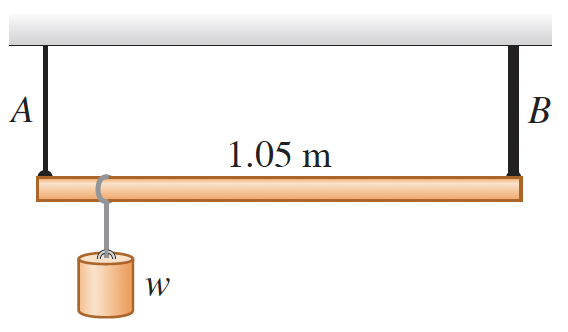
\includegraphics[width=0.5\linewidth]{../figures/P11_83.png}
  \label{fig:P11_83}
\end{figure}

A \qty{1,05}{m}-long rod of negligible weight is supported at its ends by wires $A$ and $B$ of equal length (\textbf{\autoref{fig:P11_83}}). The cross-sectional area of $A$ is \qty{2,00}{mm^2} and that of $B$ is \qty{4,00}{mm^2}. Young’s modulus for wire $A$ is \qty{1,80e11}{Pa}; that for $B$ is \qty{1,20e11}{Pa}. At what point along the rod should a weight $w$ be suspended to produce

\subsection*{(a)}
Equal stresses in $A$ and $B$?
\bigbreak
\begin{figure}[ht]
  \centering
  \incfig[0.8]{F22_11_83}
  \caption{Fritlegemediagram}
  \label{fig:F22_11_83}
\end{figure}

Først findes et udtryk for kraften i hhv. $A$ og $B$ som funktion af placeringen af vægten $w$. Vi lader $x$ betegne afstanden fra $A$'s fæstningspunkt på stangen til punktet på stangen, hvor $w$ hænger fra. Se evt. \textbf{\autoref{fig:F22_11_83}}. Vi sætter $x = 0$ til vores 0-punkt og kan derfor finde et udtryk for $F_A$ og $F_B$ med betingelserne for statik som
\[ 
\sum F_y = F_A + F_B - w = 0
\]
og
\[ 
\sum \tau = - w \cdot x + F_B \cdot l = 0
.\]
Vha. betingelsen for momenter kan vi skrive
\[ 
F_{B} = \frac{w \cdot x}{l}
.\]
Og dermed har vi at
\[ 
F_A = w - F_B = w - \frac{w\cdot x}{l} = w \left( 1 - \frac{x}{l} \right)
.\]
Dernæst kan vi fortsætte til at finde ud af hvornår de to spændinger produceret er ens. Spændingen er generelt givet som
\[ 
\sigma = \frac{F_{\perp}}{A}
.\]
Vi har altså at
\begin{align*}
  \frac{w\cdot x}{l \cdot A_B} &= \frac{w}{A_A} \left( 1 - \frac{x}{l} \right) \\
  \frac{x}{l\cdot A_B} &= \frac{1}{A_A} \left( 1 - \frac{x}{l} \right) \\
  \frac{A_A\cdot x}{l} &= A_B \left( 1 - \frac{x}{l} \right) \\
  A_A\frac{x}{l} &= A_B - A_B \cdot \frac{x}{l} \\
  A_B &= (A_A + A_B) \frac{x}{l} \\
  x &= \frac{A_B \cdot l}{A_A + A_B} \\
    &= \frac{\qty{4,00}{mm^2} \cdot \qty{1,05}{m}}{\qty{2,00}{mm^2} + \qty{4,00}{mm^2}} \\
    &= \qty{0,700}{m}  
.\end{align*}
Altså skal vægten $w$ placeres ved $x = \qty{0,700}{m}$ for at opnå ens spænding i de to reb. 



\subsection*{(b)}
Equal strains in $A$ and $B$?
\bigbreak
Vi har tidligere fundet spændingen i begge reb som funktion af placeringen af vægten $w$. Idet vi har at
\[ 
Y = \frac{\sigma}{\epsilon} \implies \epsilon = \frac{\sigma}{Y}
.\]
Kan vi omregne disse to udtryk for spændingen i hhv. $A$ og $B$ til tøjninger i hhv. $A$ og $B$. Vi får altså
\[ 
  \epsilon_A = \frac{\sigma_A}{Y_A} = \frac{w}{A_A \cdot Y_A}\left( 1 - \frac{x}{l} \right)
\]
og
\[ 
  \epsilon_B = \frac{w\cdot x}{l \cdot Y_B}
.\]
Disse to sættes lig hinanden så vi får at
\begin{align*}
  \epsilon_A &= \epsilon_B \\
  \frac{w}{A_A \cdot Y_A} \left( 1 - \frac{x}{l} \right) &= \frac{w\cdot x}{l \cdot Y_B}
.\end{align*}
Vi ser altså, at dette tilsvarer tilfældet fra (a), dog med $A$ byttet ud med $AY$. Vi får altså at løsningen bliver
\begin{align*}
  x &= \frac{A_BY_B \cdot l}{A_AE_A + A_BE_B} \\
  &= \frac{\qty{4,00}{mm^2} \cdot \qty{1,20e11}{Pa} \cdot \qty{1,05}{m}}{\qty{4,00}{mm^2} \cdot \qty{1,20e11}{Pa} + \qty{2,00}{mm^2} \cdot \qty{1,8e11}{Pa}} \\
  &= \qty{0,600}{m} 
.\end{align*}
Altså skal vægten $w$ placeres ved $x = \qty{0,600}{m}$ for at $A$ og $B$ får samme tøjning.


\section*{Opg. 11.84}
\begin{figure} [ht]
  \centering
  \caption{d}
  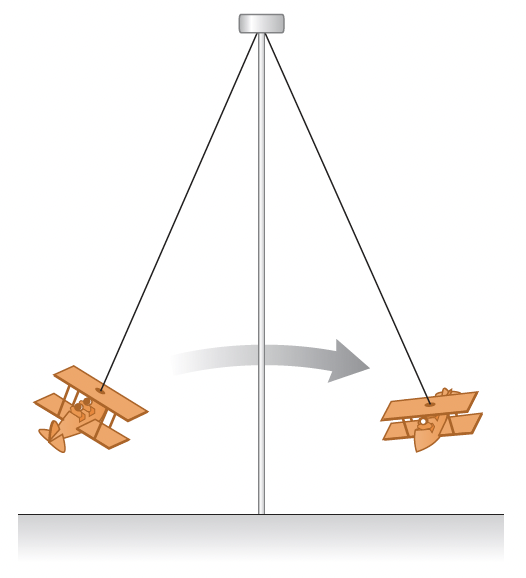
\includegraphics[width=0.5\linewidth]{../figures/P11_84.png}
  \label{fig:P11_84}
\end{figure}

An amusement park ride consists of airplane-shaped cars attached to steel rods (\textbf{\autoref{fig:P11_84}}). Each rod has a length of \qty{15,0}{m} and a cross-sectional area of \qty{8,00}{cm^2} . The rods are attached to a frictionless hinge at the top, so that the cars can swing outward when the ride rotates.

\subsection*{(a)}
How much is each rod stretched when it is vertical and the ride is at rest? (Assume that each car plus two people seated in it has a total weight of \qty{1900}{N}.)
\bigbreak
Først findes spændingen $\sigma$ som
\[ 
\sigma = \frac{F}{A} = \frac{\qty{1900}{N}}{\qty{8,00}{cm^2}} = \qty{2,375e6}{Pa} 
.\]
Youngs modul for stål er ifølge bogen $Y_{steel} = \qty{20e10}{Pa}$. Vi kan altså nu finde tøjningen i stangen som
\[ 
\epsilon = \frac{\sigma}{Y} = \frac{\qty{2,375e6}{Pa}}{\qty{20e10}{Pa}} = \num{1,1785e-5} 
.\]
Strækket i stangen $\Delta l$ kan da findes vha. definitionen af tøjningen som
\begin{align*}
  \frac{\Delta l}{l_0} &= \epsilon \\
  \Delta l &= \epsilon\cdot l_0 \\
  &= \num{1,1785e-5} \cdot \qty{15,0}{m}   \\
  &= \qty{0,177}{mm}
.\end{align*}

\subsection*{(b)}
When operating, the ride has a maximum angular speed of \qty{12,0}{rev/min}. How much is the rod stretched then?

\begin{figure}[ht]
  \centering
  \incfig[0.4]{F22_11_84}
  \caption{Fritlegemediagram}
  \label{fig:F22_11_84}
\end{figure}
\bigbreak
Med udgangspunkt i \textbf{\autoref{fig:F22_11_84}} placeres et koordinatsystem således at z-aksen går ind i papiret. Vi har da statisk ligevægt i $xy$-planet og kan derfor benytte at
\[
  \sum F_x &= F_x - F_{cp} = 0 \\
.\]
$F_x$ må være givet som
\[ 
  F_x = F\cdot \sin(\theta)
.\]
Og centripetalkraften kan findes som produktet af vognens masse og centripetalaccelerationen som
\[ 
  F_{cp} = mr\cdot \omega^2 = m \cdot l \cdot \sin(\theta) \cdot \omega^2
.\]
Først omregnes vinkelhastigheden fra \unit{rev/min} til \unit{rad/s} som
\[ 
  \qty{12,0}{\frac{rev}{min}} \cdot 2\pi \unit{\frac{rad}{rev}} \cdot \frac{1}{60} \unit{\frac{min}{s}} = \qty{1,257}{\frac{rad}{s}}  
.\]


Vi har derfor at
\begin{align*}
  F\cdot \sin(\theta) &= ml\omega^2 \cdot \sin(\theta) \\
  F &= ml\omega^2 \\
    &= \frac{\qty{1900}{N}}{\qty{9.80}{\frac{m}{s^2}}} \cdot \qty{15,0}{m} \cdot \qty{1,257}{\frac{rad}{s}}
    &= \qty{3656}{N} 
.\end{align*}
Dernæst kan spændingen $\sigma$ findes som
\[ 
  \sigma = \frac{F}{A} = \frac{\qty{3656}{N}}{\qty{8,00}{cm^2}} = \qty{4,57e6}{Pa} 
.\]
Og slutteligt kan formlen for tøjning bruges til at finde forlængelsen som
\[ 
\Delta l = \frac{\sigma \cdot l_0}{Y}
.\]
Vi får altså
\[ 
\Delta l = \frac{\qty{4,57e6}{Pa} \cdot \qty{15,0}{m}}{\qty{20e10}{Pa}} = \qty{0,34}{mm} 
.\]



\section*{Opg. 11.89}
\begin{figure} [ht]
  \centering
  \caption{d}
  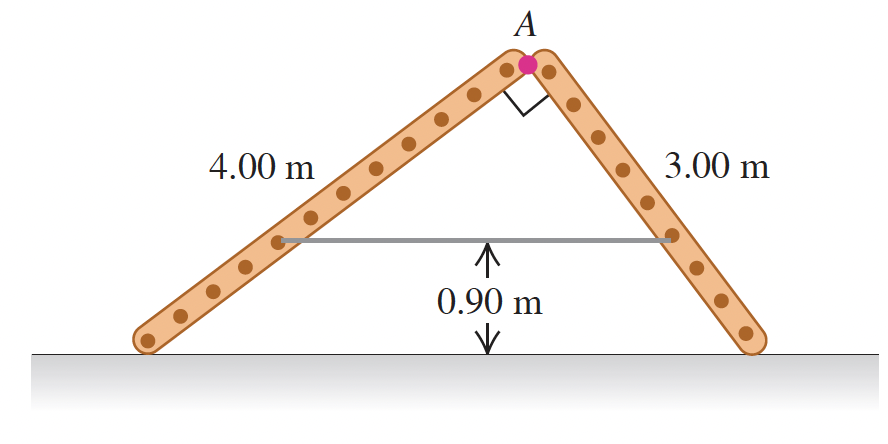
\includegraphics[width=0.5\linewidth]{../figures/P11_89.png}
  \label{fig:P11_89}
\end{figure}

Two ladders, \qty{4,00}{m} and \qty{3,00}{m} long, are hinged at point $A$ and tied together by a horizontal rope \qty{0,90}{m} above the floor (\textbf{\autoref{fig:P11_89}}). The ladders weigh \qty{480}{N} and \qty{360}{N}, respectively, and the center of gravity of each is at its center. Assume that the floor is freshly waxed and frictionless.

\subsection*{(a)}
Fund the upward force at the bottom of each ladder.

\subsection*{(b)}
Find the tension in the rope.

\subsection*{(c)}
Find the magnitude of the one ladder exerts on the other at point $A$.

\subsection*{(d)}
If an \qty{800}{N} painter stands at point $A$, find the tension in the horizontal rope.

\end{document}
